\documentclass{article}
\usepackage{tikz}
\begin{document}
	
\title{ExaGEP Plan of Work}

\author{G.~A.}

\maketitle

\section{Representation of Circuits}

\begin{figure}[h]\centering{%
	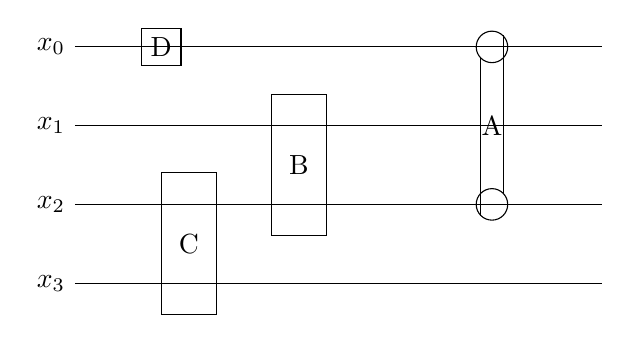
\begin{tikzpicture}
		\def\yl{-1}
		\def\xl{7}
		\node (x0) at (0,0) {$x_0$};
		\node (x1) at (0, \yl) {$x_1$};
		\node (x2) at (0, 2*\yl) {$x_2$};
		\node (x3) at (0, 3*\yl) {$x_3$};
		\coordinate (l0) at (\xl, 0);
		\coordinate (l1) at (\xl, \yl);
		\coordinate (l2) at (\xl, 2*\yl);
		\coordinate (l3) at (\xl, 3*\yl);
		\draw (x0) -- (l0);
		\draw (x1) -- (l1);
		\draw (x2) -- (l2);
		\draw (x3) -- (l3);
		\node[rectangle,draw=black] at (0.2*\xl, 0) {D};
		\draw (0.4*\xl, 0.6*\yl) -- (0.5*\xl, 0.6*\yl) -- (0.5*\xl, 2.4*\yl) -- (0.4*\xl, 2.4*\yl) -- cycle;
		\node at (0.45*\xl, 1.5*\yl) {B};
		\draw (0.2*\xl, 1.6*\yl) -- (0.3*\xl, 1.6*\yl) -- (0.3*\xl, 3.4*\yl) -- (0.2*\xl, 3.4*\yl) -- cycle;
		\node at (0.25*\xl, 2.5*\yl) {C};
		\node[circle, draw=black, minimum size=0.4cm] (A0) at (0.8*\xl, 0) {};
		\node[circle, draw=black, minimum size=0.4cm] (A1) at (0.8*\xl, 2*\yl) {};
		\draw (A0.south west) -- (A1.south west);
		\draw (A0.north east) -- (A1.north east);
		\node at (0.8*\xl, \yl) {A};
	\end{tikzpicture}}
	\caption{\label{fig:circuit}
		An example of a 4-bit quantum circuit with gates A, B, C, and D in order
		to explain the circuit encoding in genetic expression programming.}
\end{figure}

The 4-bit quantum circuit in Fig.~\ref{fig:circuit} will be represented
by the following four genes A$_0$ D$x_0$  B$_1x_1$ C$_0x_2x_3$;
 B$_0x_1$ C$_0x_2x_3$; A$_1$B$_1x_1$C$_0x_2 x_3$; and C$_1x_2x_3$.
Here, A, B, C, and D are gates, the input is to the left, and the output to the right.


To understand the first gene, consider that it is the first output of applying
the quantum circuit to the ket $|x_0, x_1, x_2, x_3\rangle$. Therefore, we need
to apply the first output of gate A, indicated by A$_0$ to two inputs, because
gate A takes two inputs. The first input is the result of applying the D gate
to $x_0$ so we have the first part as A$_0$ D$x_0\ldots$. The second input to gate
A is the second output of B or B$_1$. Now B has two inputs, one is $x_1$ and the other is
the first output of gate C, which we denote by C$_0$. Combining it all we have so far
A$_0$ D$x_0$ B$_1x_1$C$_0\ldots$. Finally, gate C takes to inputs which are $x_2$ and $x_3$,
yielding the first output or first gene as A$_0$ D$x_0$ B$_1x_1$C$_0x_2x_3$.

\section{Optimization Procedure}
Given a state $|\psi^{\textrm{known}}\rangle$, we want to find a quantum
circuit that generates it for an initial state $|\psi_0\rangle$
\begin{enumerate}
	\item Start with an original population of $M=100$ circuits generated randomly.
	\item Start with a pure state ket of length $N$: $|\psi_0\rangle\equiv|x_0, x_1, \ldots, x_{N-1}\rangle$.
	\item By genetic expression programming mutations and combinations of the original 
	population created in step 1, generate $M'=200$ new circuits
	$\{\mathcal{C}(\varphi)\}_{0\le j<M}$, optionally dependent on $K$ continuous variables
	$\varphi\equiv\{\varphi_0, \varphi_1, \cdots, \varphi_{K-1}\}$.
	\item For every circuit $j$, define the $\varphi-$dependent ket $\psi_j(\varphi)=\mathcal{C}_j(\varphi)|\psi_0\rangle$.
	\item For every circuit $j$, define the pre-fitness $P_j$ function by
	\begin{equation}
		P_j(\varphi) = |\langle \psi^{\textrm{known}} | \psi_j(\varphi)\rangle|^2
	\end{equation}
	and find the $\varphi$ where the maximum occurs; let's call it $\varphi_{\textrm{max}}$.
	\item For every circuit $j$, calculate its fitness $F_j = P_j(\varphi_{\textrm{max}})$.
	\item Eliminate the $M'-M=100$ circuits with less fitness and keep the others.
	\item Go to step 3. 
\end{enumerate}
\end{document}